\documentclass[12pt,letterpaper,oneside]{book}
%%%%%%%%%%%%%%%%%%%%%%%%%%%%%%%%%%%%%%%%%%%
%%%%%%% Lugar de los package
%%%%%%%%%%%%%%%%%%%%%%%%%%%%%%%%%%%%%%%%%%%
\usepackage[right=2.5cm,left=2.5cm,top=2.5cm,bottom=2.5cm]{geometry}%márgenes de la pagina
\usepackage{fancyhdr}
\usepackage{tikz}
\usepackage[spanish,es-noshorthands,es-lcroman,es-tabla]{babel}
\usepackage[spanish]{translator}
\usepackage[utf8]{inputenc}
\usepackage{graphicx}
%\usepackage{multicol} %multicolumnas
\usepackage{subfigure} %incluir multiples imágenes en una figura
% \usepackage[vlined, lined, linesnumbered, algosection]{algorithm2e} %paquete para los algoritmos en pseudocódigo
\usepackage{enumerate} %permite cambiar el item de la enumeración mas fácilmente: 
\usepackage{amsmath, amsthm, amssymb}
\usepackage{lscape}
\usepackage{pdflscape}
						%Otra opción renombrar el item: \renewcommand{\labelenumi}{\Alph{enumi}.}
\RequirePackage{url} %citación de URL
\usepackage{hyperref}
\usepackage{longtable}
\usepackage{listings}
\usepackage{float}

%%%%%%%%%%%%%%%%%%%%%%%%%%%%%%%%%%%%%%%%%%%%%%%%%%%%%%%%%%%%%%%%%%%
%%%%%%% Definción de Estilos de los títulos de la figuras y tablas
%%%%%%%%%%%%%%%%%%%%%%%%%%%%%%%%%%%%%%%%%%%%%%%%%%%%%%%%%%%%%%%%%%%

\makeatletter
%%Tables and Figures

\long\def\@makecaption#1#2{%
   \vskip 10\p@
   \setbox\@tempboxa\hbox{#1. #2}%
   \ifdim \wd\@tempboxa >\hsize
       #1. #2\par
     \else
       \hbox to\hsize{\hfil\box\@tempboxa\hfil}%
   \fi
   \vskip 10\p@}

\def\thefigure{\@arabic\c@chapter.\c@figure}

\def\fps@figure{tbp}
\def\ftype@figure{1}
\def\ext@figure{lof}
\def\fnum@figure{{\bf\figurename~\thefigure}}
\def\figure{\@float{figure}}
\let\endfigure\end@float
\@namedef{figure*}{\@dblfloat{figure}}
\@namedef{endfigure*}{\end@dblfloat}

\def\thetable{\@arabic\c@table}

\def\fps@table{tbp}
\def\ftype@table{2}
\def\ext@table{lot}
\def\fnum@table{{\bf\tablename~\thetable}}
\def\table{\@float{table}}
\let\endtable\end@float
\@namedef{table*}{\@dblfloat{table}}
\@namedef{endtable*}{\end@dblfloat}

\renewcommand{\thefigure}{\thechapter.\arabic{figure}}
\renewcommand{\thetable}{\thechapter.\arabic{table}}

\def\thelstlisting{\@arabic\c@chapter.\@arabic\c@lstlisting}
\def\fnum@lstlisting{{\bf\lstlistingname~\thelstlisting}}
\makeatother

%%%%%%%%%%%%%%%%%%%%%%%%%%%%%%%%%%%%%%%%%%%%%%%%%
%%%%%%% Nombre de títulos en español con babel
%%%%%%%%%%%%%%%%%%%%%%%%%%%%%%%%%%%%%%%%%%%%%%%%%

\renewcommand{\spanishrefname}{Referencias}
\renewcommand{\spanishbibname}{Bibliograf\'{\i}a}
\renewcommand{\spanishabstractname}{Resumen}
\renewcommand{\spanishcontentsname}{\'{I}ndice}

%%%%%%%%%%%%%%%%%%%%%%%%%%%%%%%%%%%%%%%%%%%
%%%%%%% Estilo de la páginas y encabezados
%%%%%%%%%%%%%%%%%%%%%%%%%%%%%%%%%%%%%%%%%%%
\pagestyle{fancy}
\pagestyle{headings} %Se puede seleccionar esta opción o todas las anteriores.


\renewcommand{\headrulewidth}{0pt} % grosor de la línea de la cabecera
\linespread{1.5} %interlineado

%\begin{enumerate}[(a)] %for small alpha-characters within brackets.
%\setlength{\parindent}{12pt}
%\setlength{\parindent}{1.5em}
%\setlength{\parindent}{2cm}

\begin{document}

\thispagestyle{empty}

\frontmatter
\begin{center}
\begin{Large}
\vspace*{0.4in}
\vspace*{2in}
\textbf{MEDICIÓN DE RESISTIVIDAD DEL SUELO}
\textbf{UCV}
\end{Large}
\vspace*{0.3in}
\end{center}
% \rule{80mm}{0.1mm}\\
\vspace*{2in}

\begin{flushright}
Br. Escobar, Caleb\\
C.I.: 24.898.930
\end{flushright}

\vspace*{0.3in}
\begin{center}
    Caracas, 2024
\end{center}

\newpage
%\addtocounter{page}{6}
%índice
\tableofcontents
\listoffigures
\listoftables

\mainmatter
%%%%%%%%%%%%%%%%%%%%%%%%%%%%%%%%%%%%%%%%%%%%%%%%%%%%%%%%%%
%%%%              INTRODUCCIÓN                   %%%%%%%%%
%%%%%%%%%%%%%%%%%%%%%%%%%%%%%%%%%%%%%%%%%%%%%%%%%%%%%%%%%%
\chapter{INTRODUCCIÓN}
xxx


\chapter{Metodología}

\section{Localización}
Se realizó un estudio de suelo en Frente de la facultad de arquitectura, UCV, la cual tiene la siguiente localización ( $10.489040^{\circ}, -66.887290^{\circ}$). Tomando como referencia los datos de Google Earth.

\begin{figure}[H]
    \centering
    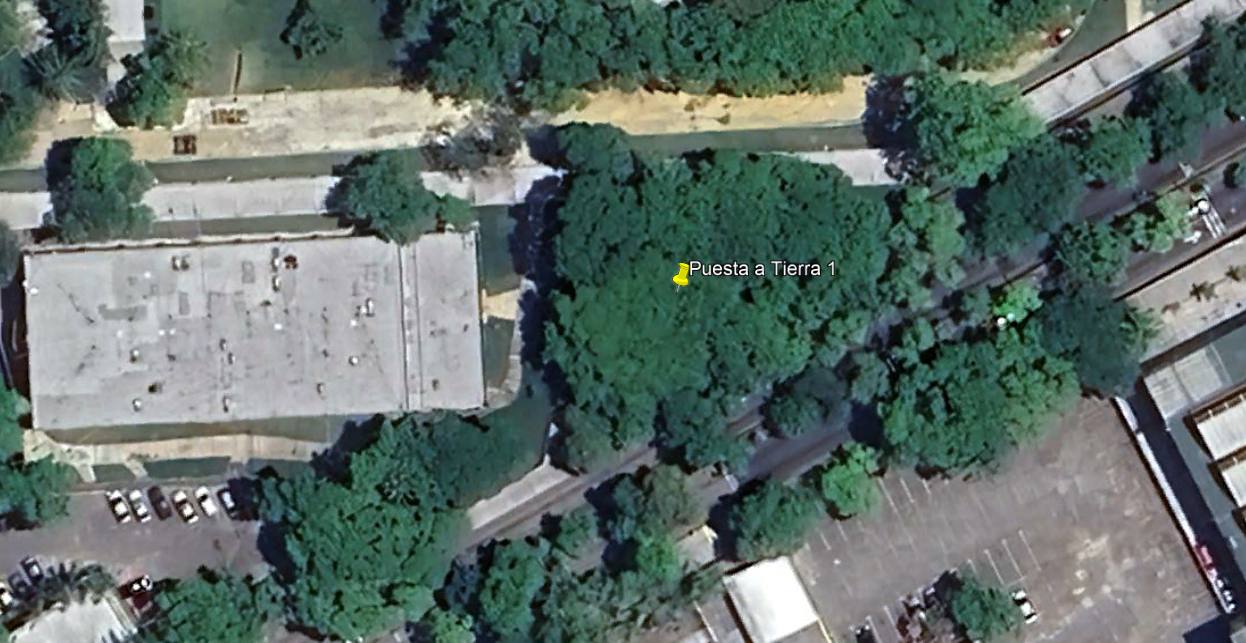
\includegraphics[scale=0.6]{Imagenes/localizacion.png}
    \caption{Localización}
    \label{local}
   \end{figure}

\section{Equipos}
\section{Medición de resistencia}
\chapter{Memoria Descriptiva}

\section{Ubicación}

\section{Resistencia}
\begin{table}[H]
    \centering
    \caption{Me}
    \begin{tabular}{|c|c|c|c|c|} 
    \hline
    \textbf{Medidas} & \textbf{Separación c} & \textbf{Separación d} & \textbf{Resistencia medida} & \textbf{Resistividad aparente}  \\ 
    \hline
    1                & 1                     & 1                     & 7,5                         &                                 \\
    2                & 1,5                   & 1,5                   & 3,75                        &                                 \\
    3                & 2                     & 2                     & 1,4                         &                                 \\
    4                & 2,5                   & 2,5                   & 1,05                        &                                 \\
    5                & 3                     & 3                     & 0,85                        &                                 \\
    6                & 4                     & 4                     & 0,65                        &                                 \\
    7                & 5                     & 5                     & 0,5                         &                                 \\
    \hline
    \end{tabular}
    \end{table}
\chapter{Memoria de Cálculo}

%\input{Capitulos/Cap5/Cap5.tex}



\end{document}